%%%%%%%%%%%%%%%%%%%%%%%%%%%%%%%%%%%%%%%%%%%%%%%%%%%%%%%%%%%%%%%%%%%%%%%%
% ParityMem -- minimal submission polish v7, 2026-09-10.
% Figure labels and manuscript share one vocabulary; frozen scientific records unchanged.
% Artwork: original vector Form XObjects extracted from the user-selected PDF7.
% No model/backend/GPU or new timing measurement; raw evidence unchanged.
% Base ZIP sha256: faeaf15ef1aba93c5f1a1ca7da688bd5e9216d0cbce91f79c9aad62b6fcebf75
% All bibliography entries are maintained in references.bib.
% Added balanced accuracy is calculated only from the audited binary endpoints.
% Table 1: bound sealed Full, existing post-hoc baselines, historical aggregate components.
% No server merge, new inference, or reconstruction of missing severity labels.
% Text base: CompactPair (2026-09-06), with main.tex lineage from 2026-09-03.
% Artwork: native academic-figure reflow of approved photo cutouts; see revision_audit/.
% Main: main.tex | Engine: pdfLaTeX | Bibliography: BibTeX.
% See README_zh.md and revision_audit/ for provenance and author checks.
%%%%%%%%%%%%%%%%%%%%%%%%%%%%%%%%%%%%%%%%%%%%%%%%%%%%%%%%%%%%%%%%%%%%%%%%
\documentclass[letterpaper]{article}
\usepackage{spconf}
\usepackage{amsmath}
\usepackage{booktabs}
\usepackage{capt-of}
\usepackage{cite}
\usepackage{cuted}
\setlength{\stripsep}{3pt plus 1pt minus 1pt}
\usepackage{multicol}
\usepackage{graphicx}
\usepackage{microtype}
\usepackage{tabularx}
\usepackage{xspace}
\usepackage{xurl}
\usepackage[hidelinks]{hyperref}
\hypersetup{
  pdftitle={ParityMem: Semantic Compatibility Prediction for Structured LLM Inference},
  pdfsubject={Semantic compatibility and reliable evaluation of structured LLM inference},
  pdfkeywords={semantic compatibility, structured LLM inference, tool-using agents, inference backends, evaluation validity}
}

\newcommand{\system}{\textsc{ParityMem}\xspace}
\newcommand{\contractir}{\textsc{ContractIR}\xspace}
\newcolumntype{Y}{>{\raggedright\arraybackslash}X}
\newcounter{auditprocedure}
\hyphenation{Bench-Guard bench-marks au-dit-ing back-end}

\title{ParityMem: Semantic Compatibility Prediction for Structured LLM Inference}
% AUTHOR ACTION REQUIRED: fill real names and affiliations before submission.
\name{Authors to be confirmed}
\address{Affiliation and email pending author confirmation}

\begin{document}
\ninept
\emergencystretch=11pt
\onecolumn
\raggedbottom
\setlength{\multicolsep}{4pt}
\maketitle
% Two independent compact figures, each exactly one column wide; same height as Fig. 3.
\noindent
\begin{minipage}[t]{\dimexpr(\textwidth-\columnsep)/2\relax}
  \vspace{0pt}
  \begin{minipage}[t][225pt][t]{\linewidth}
\begin{abstract}
Comparing backends for tool-using LLMs requires separating interface effects
from model behavior: benign ID rewrites may look different, while locally valid
calls can block continuation. \system predicts compatibility and localizes
source-supported consumer violations before outcome inspection. Pairs with
validated compatibility and reachability are admitted; within-backend stability
precedes canonical-action comparison. Across 354 version-pinned trace--model--backend
cells, \system accepts all 295 safe cells and detects all 59 blocked cells.
A new adapter and contract reuse the frozen checking core on 144 trace--contract
conditions (48 traces $\times$ 3 contracts), matching validation. Among
36 admitted backend pairs, five runs per backend yield 33 pairs with the
same canonical action and 3 stable differences. Median recurring audit latency
is 3.94~ms over 7,200 timed repetitions of 72 decisions, excluding contract
specification and model inference. Together, these results make interface validity
explicit, support reuse across source-specific contracts, and expose stable
action differences while preserving permitted variation.

\end{abstract}

\begin{keywords}
semantic compatibility, structured LLM inference, tool-using agents,
inference backends, evaluation validity
\end{keywords}
  \end{minipage}
  \par\vspace{3pt}
  \centering
  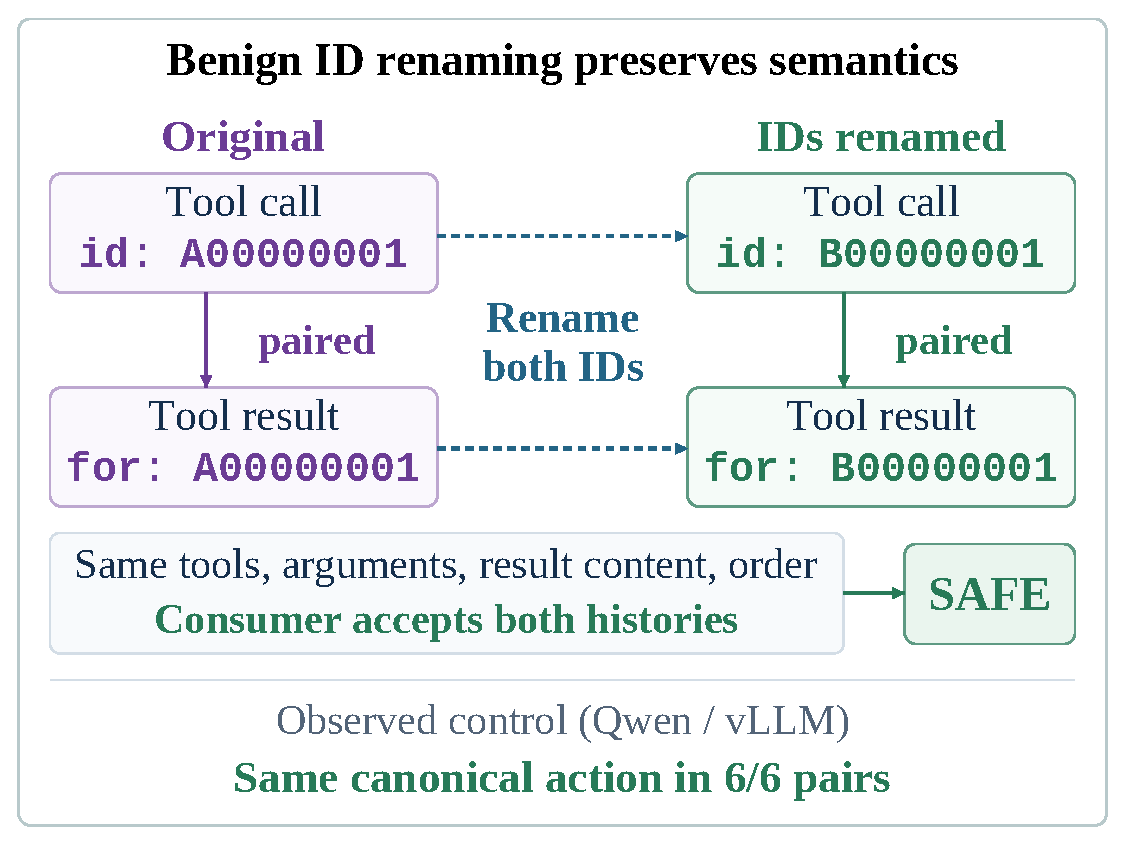
\includegraphics[width=\linewidth]{figures/figure1_tool_use_loop_compact.pdf}
  \captionof{figure}{Benign ID renaming preserves semantics. Jointly renaming
  a call ID and its result reference preserves pairing, content, order and consumer acceptance.
  All 6/6 Qwen/vLLM within-backend control pairs retain the same canonical action.}
  \label{fig:loop}
\end{minipage}\hfill
\begin{minipage}[t]{\dimexpr(\textwidth-\columnsep)/2\relax}
  \vspace{0pt}
  \begin{minipage}[t][225pt][t]{\linewidth}
\section{Introduction}
Reliable evaluation of structured LLM inference must distinguish model
behavior from interface effects. Benchmarks such as $\tau$-bench, ToolBench
(introduced in ToolLLM), and AppWorld define tasks~\cite{yao2024tau,qin2024toolllm,trivedi2024appworld}.
Model-specific dialog protocols structure tool interactions~\cite{grattafiori2024llama3},
while template mismatches can affect behavior~\cite{jiang2025chatbug}.
Serving systems including vLLM and SGLang~\cite{kwon2023vllm,zheng2024sglang}
impose runtime acceptance conditions.

Figure~\ref{fig:loop} shows that consistent ID renaming can preserve an
interaction despite different strings. Figure~\ref{fig:next-turn-closure}
shows that parsing, execution, and pairing can succeed while the next-history
consumer rejects the turn. Literal equality flags the benign rewrite;
local schema validity misses the continuation failure.

\system answers three questions before attributing output differences to
model behavior: \textbf{(i)} Is each trace contract-compatible despite benign
representation changes? \textbf{(ii)} For a source-supported defect, which
consumer obligation fails first and what consequence is demonstrated?
\textbf{(iii)} If both sides are validated and reachable, do their stable
canonical actions agree?

  \end{minipage}
  \par\vspace{3pt}
  \centering
  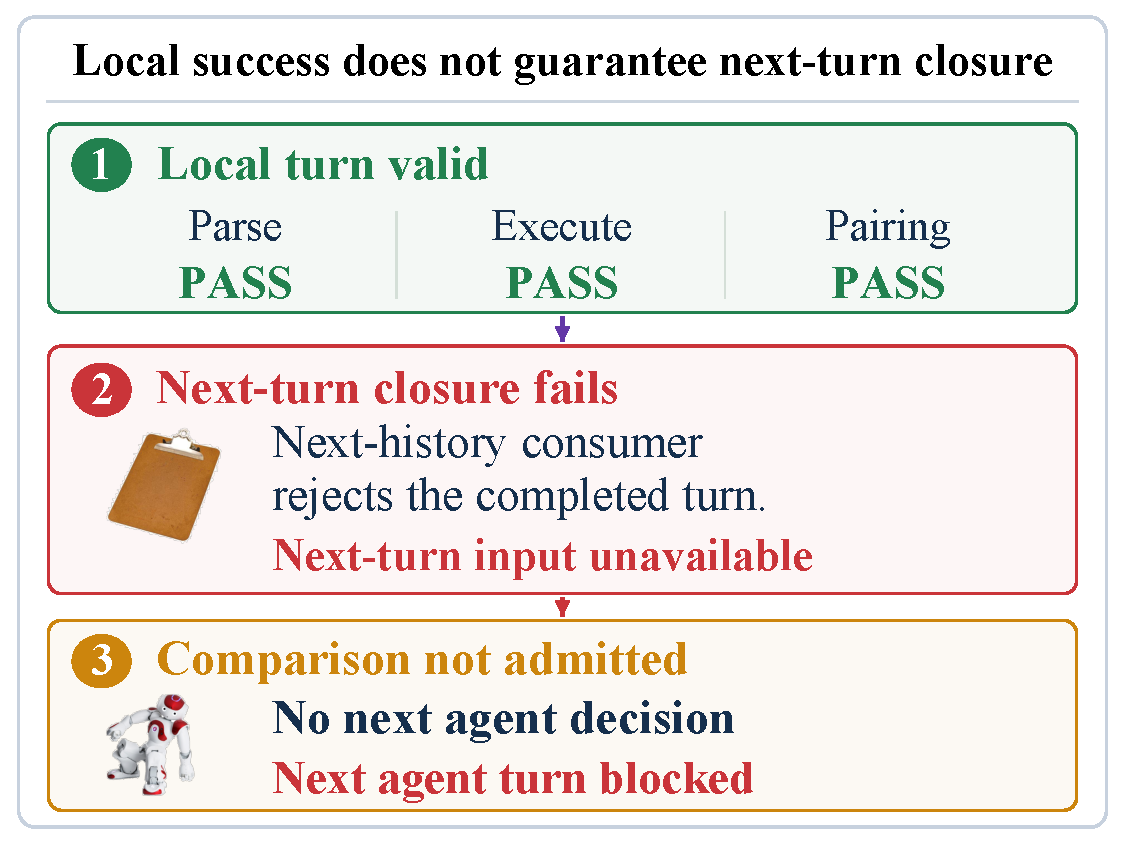
\includegraphics[width=\linewidth]{figures/figure2_f1_motivation_compact.pdf}
  \captionof{figure}{Local success does not guarantee next-turn closure.
  Parsing, execution and pairing succeed, but the next-history consumer
  rejects the completed turn.}
  \label{fig:next-turn-closure}
\end{minipage}

\par\vspace{8pt}
\begingroup
\setlength{\multicolsep}{0pt}
\setlength{\premulticols}{0pt}
\setlength{\postmulticols}{0pt}
\begin{multicols}{2}
\noindent
Tool Playgrounds evaluates tool interaction; WTU-EVAL evaluates tool-use
necessity~\cite{dong2025toolplaygrounds,liu2025wtueval}. AgentSuite, BenchGuard,
and Auto Benchmark Audit~\cite{suh2026agentsuite,tu2026benchguard,wang2026aba}
audit specifications, environments, ground truths and evaluators.
AgentRx~\cite{barke2026agentrx} localizes failure steps;
\mbox{HarnessFix}~\cite{chen2026harnessfix} diagnoses and repairs harness flaws.
\system makes \emph{comparison admissibility} explicit: source-grounded checks preserve
permitted rewrites (Fig.~\ref{fig:loop}) and diagnose consumer violations
(Fig.~\ref{fig:next-turn-closure}), admitting validated, reachable pairs for
stable action comparison.
\end{multicols}
\endgroup

\clearpage
% Paper Figure 3 keeps the accepted structure/assets with enlarged, reflowed labels.
\twocolumn[{
\begin{minipage}{\textwidth}
  \centering
  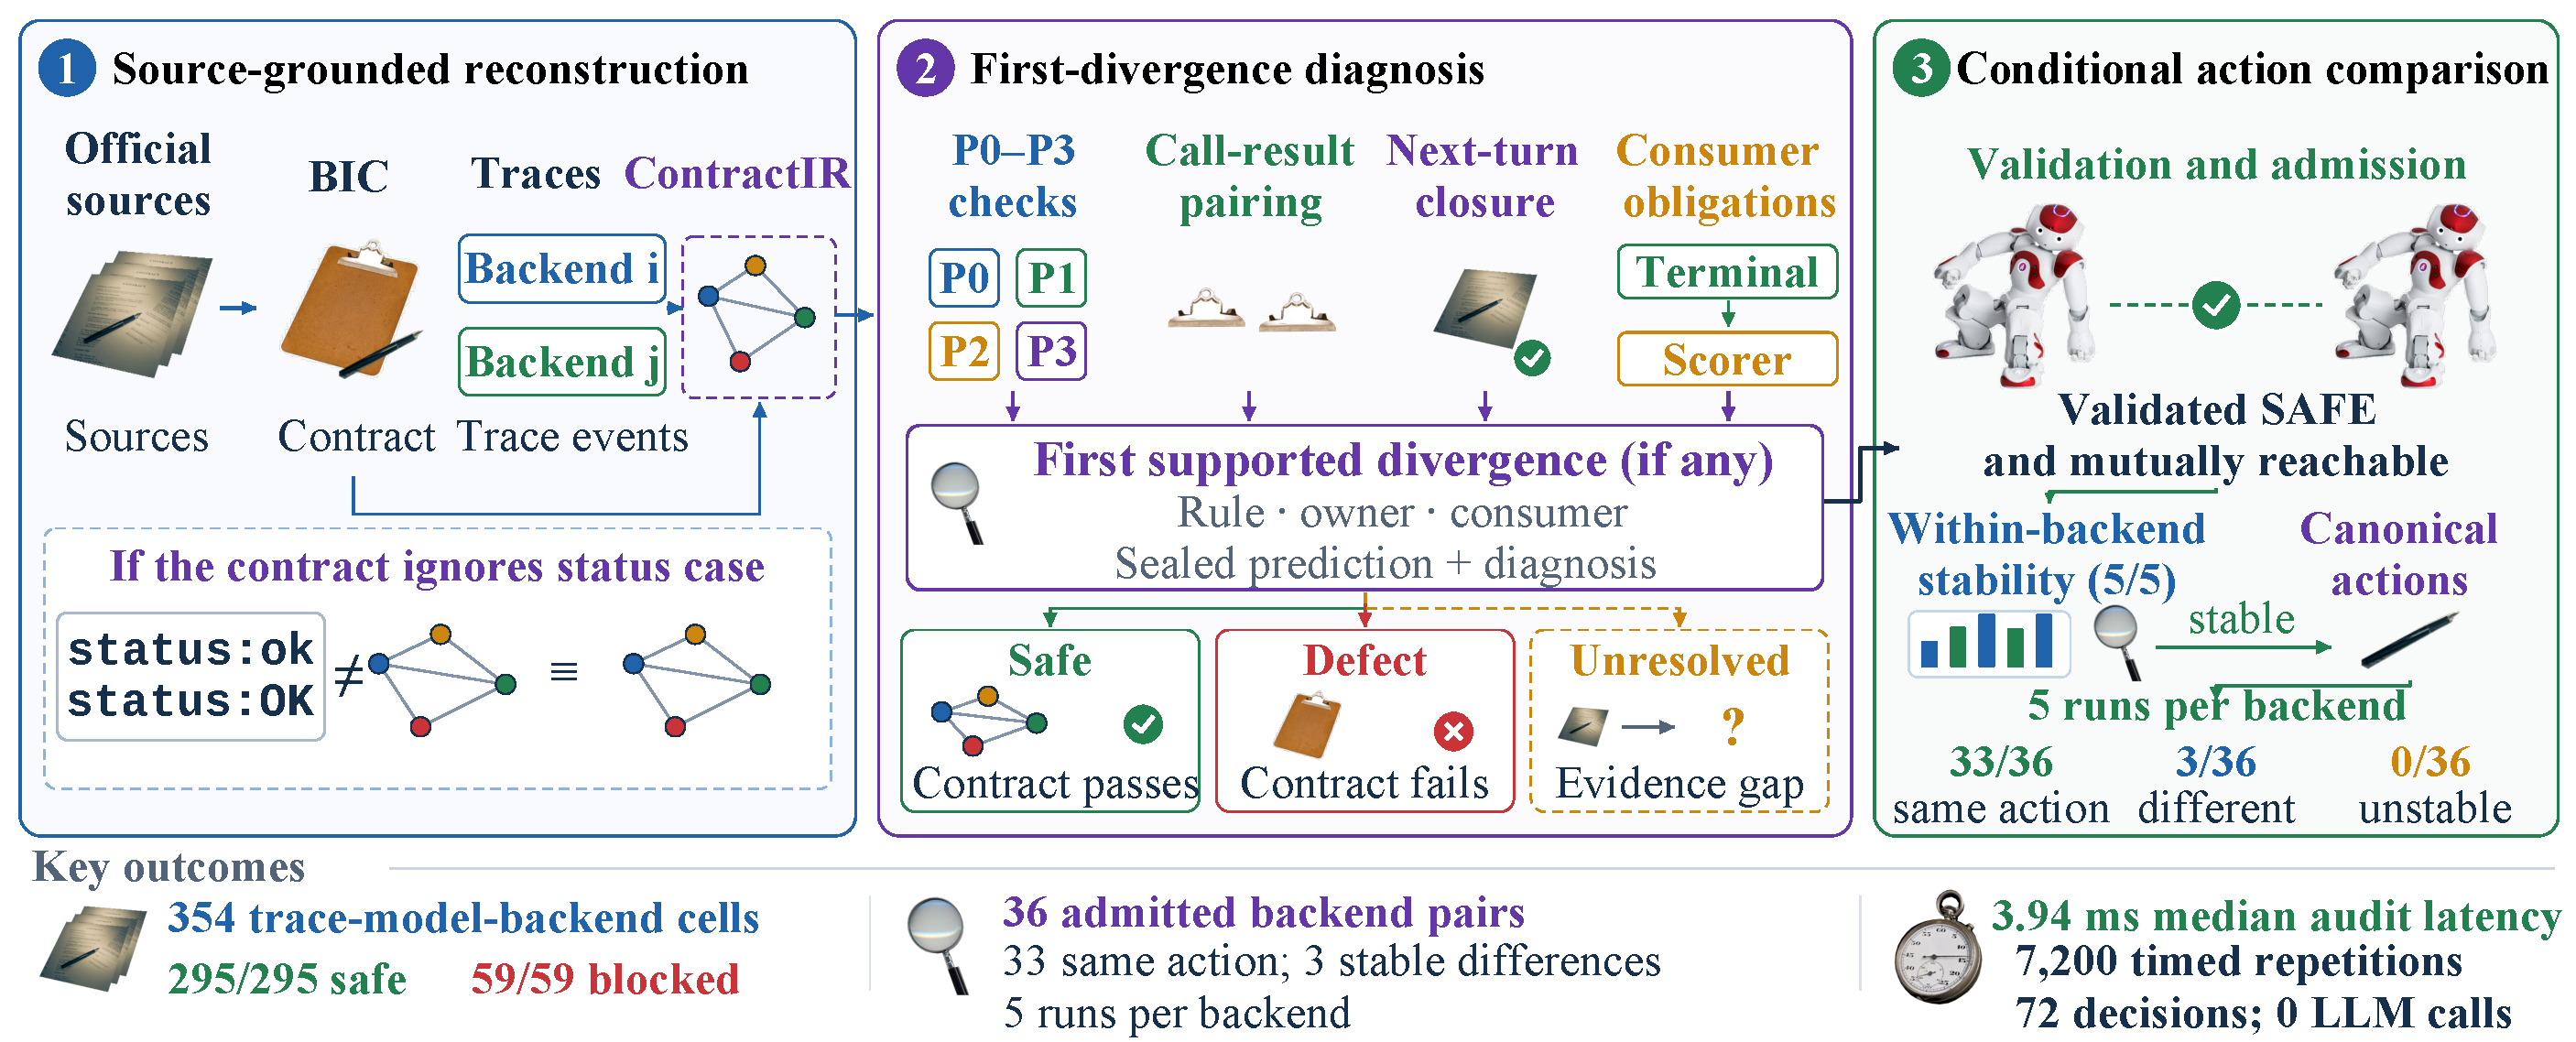
\includegraphics[width=\textwidth]{figures/figure3_method_overview.pdf}
  \captionof{figure}{\system: source-grounded reconstruction, first-divergence
  diagnosis, and conditional action comparison. Predictions are sealed;
  officially validated \textsc{Safe} and consumer reachability admit pairs. Within-backend
  5/5 stability precedes canonical-action comparison. Bottom: 354 trace--model--backend
  cells, 36 admitted backend pairs, and recurring audit latency from 7,200 timed
  repetitions over 72 decisions.}
  \label{fig:overview}
\end{minipage}
\vspace{10pt}
}]

\section{Compatibility-first comparison}
\system supports comparison admission with compatibility verdicts and
source-linked diagnoses (Fig.~\ref{fig:overview}). For each supported defect,
the record identifies the violated predicate, its owner and consumer,
the first divergence, and the strongest demonstrated consequence.

\subsection{Source-grounded reconstruction}
For interaction $x$ and backend $b$, authoritative sources $\mathcal S_x$
define a behavioral interface contract (BIC) $C_x$ governing the structured
trace $T_{b,x}$:
\begin{equation}
 C_x=\operatorname{BIC}(\mathcal S_x),\qquad
 I_{b,x}=\operatorname{ContractIR}(T_{b,x};C_x).
 \label{eq:objects}
\end{equation}
Each obligation specifies its source and version, owner, consumer, and acceptance condition.
Source contracts supply integration-specific domains and predicates; record
adapters populate shared \contractir fields. Pairing, projection checks, and
source-attributed diagnosis operate over those fields. Human review confirms
source authority and precedence, enabling repeatable automatic checks
across histories.

\contractir retains raw and semantic forms of typed messages, calls,
arguments, results, transitions, and identifier/scorer bindings, with order,
owner, provenance, and consumer. Transport-ID renaming preserves meaning when
it retains the call--result bijection and consumer acceptance. For a
contract-relevant projection $\Pi_{C_x}$ and next consumer $N_{C_x}$,
a benign change $\phi$ satisfies
\begin{equation}
 \Pi_{C_x}(T)=\Pi_{C_x}(\phi(T)),\quad
 \{T,\phi(T)\}\subseteq\operatorname{Dom}(N_{C_x}).
 \label{eq:equiv}
\end{equation}
Equation~\eqref{eq:equiv} defines admissible representation freedom;
diagnostic probes restore a target acceptance condition while preserving
the specified semantic projection and non-target obligations.

The audited SGLang--Mistral path illustrates identifier-domain non-closure
and source ownership:
SGLang emits a 29-character action ID, whereas the exact Mistral template
requires a nine-character alphanumeric result-binding ID~\cite{mistralai_v03_modelcard}.
The ID domain belongs to the consumer contract; the binding and order checks
remain shared. An admissible remap is collision-safe and injective, preserving
call--result correspondence, tools, arguments, order, and state.

\subsection{First-divergence diagnosis}
Cross-turn compatibility requires the next consumer to accept the completed history. On $I_{b,x}$, P0 checks representability;
P1 checks model- and benchmark-visible meaning; P2 checks actions,
authoritative state transitions, and continuation; P3 checks terminal state
and scorer-facing bindings. These projections check distinct obligations.

Pairing verifies unique call--result correspondence across transport,
execution, and model-visible IDs. For the next-history serializer $H_x$,
closure checks $T_{b,x}\in\operatorname{Dom}(H_x)$ and preserves the relevant
\contractir projection on the round trip.
The frozen contract, versions, and recorded path define the audit scope.

The checker attributes violations to source predicates and returns the
first source-supported divergence in recorded interaction/consumer order, not
P0--P3 evaluation order. Manifestations of the same predicate share one root.
The sealed prediction is
$\widehat V_{b,x}=J(C_x,I_{b,x})\in
\{\textsc{Safe},\textsc{Defect},\textsc{Unresolved}\}$:
\textsc{Safe} requires all applicable obligations to pass with sufficient
evidence; \textsc{Defect} identifies a reproducible source-supported violation;
\textsc{Unresolved} preserves uncertainty in authority or applicability.
Consequence R2 records changed model-visible meaning, R3 a demonstrated
pairing, state, or continuation effect, and R4 an observed scorer/task effect.
Verdict and reachability remain separate: altered content may still allow
execution to continue.

The case in Fig.~\ref{fig:next-turn-closure} contains three paired calls:
\texttt{get\_order}, \texttt{get\_policies}, and \texttt{process\_refund},
returning order, policy, and preview results. Parsing, pairing, and
current-turn execution succeed, but the Llama next-history cardinality guard
rejects the completed turn (R3). A projection-preserving probe restores
reachability from 0/3 to 3/3, with actual continuation in 3/3; these fractions
count per-root probe outcomes.
Prediction targets next-history acceptance from the completed turn before
inspecting that consumer's validation outcome.

Figure~\ref{fig:loop} preserves both the semantic projection and consumer
acceptance in Eq.~\eqref{eq:equiv}; Figure~\ref{fig:next-turn-closure} fails
next-turn closure despite local success.

\newpage
\subsection{Conditional action comparison}
Compatible interfaces can produce different actions. Let $A_{b,x}$ denote
status after official validation and $r_{b,x}=1$ required-consumer reachability.
Validation updates $A_{b,x}$, not the sealed prediction $\widehat V_{b,x}$.
A pair is admitted when
\begin{equation}
 E_{i,j,x}=\mathbf 1\!\left[
 A_{i,x}=A_{j,x}=\textsc{Safe}\ \land\ r_{i,x}=r_{j,x}=1\right].
 \label{eq:gate}
\end{equation}
Admitted pairs require 5/5 stability within each backend before action comparison.
Identifiers are retained for contract and pairing checks; after admission,
canonical actions omit permitted transport IDs and encode kind and ordered
(tool, argument) entries. We decode JSON argument strings and sort object keys,
preserving array order and string values, including code.
Nonempty outputs without accepted calls map to \textsc{NoTool};
parser errors and empty outputs are invalid. Execution equivalence and task
scores remain separate endpoints.

\begin{center}
\begin{minipage}{\linewidth}
\refstepcounter{auditprocedure}\label{alg:comparison}
\hrule height 0.4pt\vspace{3pt}
\noindent\textbf{Algorithm \theauditprocedure. Compatibility-first comparison}\par
\noindent\textit{Input:} confirmed contracts and recorded traces.\par
\begin{list}{\arabic{enumi}.}{\usecounter{enumi}%
\setlength{\leftmargin}{1.4em}\setlength{\labelsep}{0.4em}%
\setlength{\topsep}{1pt}\setlength{\itemsep}{0pt}%
\setlength{\parsep}{0pt}\setlength{\partopsep}{0pt}}
\item Lift each trace into its contract-conditioned \contractir.
\item Check P0--P3, pairing, and history-closure obligations.
\item Select the first source-supported violation, if any.
\item Seal each prediction and its source-linked diagnostic record.
\item Obtain official validation and required-consumer reachability.
\item Admit pairs satisfying Eq.~\eqref{eq:gate}.
\item Test five-run stability; compare the stable canonical modes.
\end{list}
\vspace{2pt}\hrule height 0.4pt
\end{minipage}
\end{center}

\section{Experiments}

\subsection{Experimental setup and validation protocol}
A matrix cell specifies a benchmark, trace, model/revision, and backend/version.
Mechanism probes count distinct roots; an adapter condition is one
trace--contract combination. An admitted backend pair fixes benchmark,
trace and model revision, with both paths validated \textsc{Safe} and required
consumers reachable. Denominators are never pooled.

Policies are frozen Qwen3-14B, Llama-3.1-8B-Instruct, and
Mistral-7B-Instruct-v0.3 revisions~\cite{yang2025qwen3,grattafiori2024llama3,jiang2023mistral7b}.
They consume official histories and tool schemas from $\tau^3$-bench and
AppWorld~\cite{tau3bench2026,yao2024tau,trivedi2024appworld} via SGLang or vLLM.
Original backend conditions fix weights, tokenizer, model-specific template,
semantic history, tool schemas and generation parameters (temperature zero).
The companion's \texttt{START\_HERE.md} lists exact revisions. \system invokes
no LLM; inference is reserved for behavioral validation.

Table~\ref{tab:compatibility} separates sealed Full, post-hoc compatibility
baselines and aggregate-derived components; adjacent systems are discussed by
task and output. On frozen record pairs, raw equality retains IDs; schema checks
types/tool names; normalization decodes JSON and removes IDs without reordering.
Rules use no outcome labels or \system logic; 1,062 per-cell baseline outputs
are scored against frozen official outcomes.

In controlled suites, \system preserves 280/280 clean replays, detects
120/120 mutations, satisfies 100/100 safe and 100/100 unsafe metamorphic
relations, and correctly classifies 300/300 blind holdout cases, including the
120/120 novel-composition subset. The source-derived holdout generator/gold
program imports no \system prediction logic, and the prediction runner has
no gold access. An independent programmatic adjudicator, with no gold access or checker imports,
agrees on class, consequence, and first divergence for 60/60 sampled cases. The companion provides the frozen core and recorded inputs for these controls.

\subsection{Compatibility accuracy and diagnostic value}
The original matrix uses SGLang~0.5.6.post2 and vLLM~0.23.0. Of 60 sampled
histories, 59 are eligible across three models and two backends (354 cells);
one AppWorld history is inapplicable in all six settings. Full predictions
precede official parser/template outcomes. Full \system matches 354/354 binary
verdicts, 59/59 R3 labels, and 354/354 first-divergence labels. All 59 blocks
reflect identifier-domain non-closure; this matrix has no R2 or unresolved cases.

\begin{strip}
\captionof{table}{Frozen matrix: 354 cells (295 safe, 59 blocked). Full:
sealed per-cell predictions; baselines: post-hoc frozen records.
$\ddagger$: historical component summaries from stratum counts.
Consequence scoring: 59 R3 blocks (demonstrated pairing, state or continuation
effects). First divergence: 295 \textsc{None}; 59 identifier-domain non-closure.
N/A: no emitted per-cell label.}
\label{tab:compatibility}
\centering
\setlength{\tabcolsep}{4.1pt}
\renewcommand{\arraystretch}{1.05}
\begin{tabular}{@{}lccccc@{}}
\toprule
Method / variant & \shortstack{Binary verdict\\correct} & \shortstack{Safe cells\\falsely flagged} & \shortstack{Blocked cells\\detected} & \shortstack{Consequence label\\correct (R3)} & \shortstack{First-divergence\\correct} \\
\midrule
\multicolumn{6}{@{}l}{\textit{Offline record baselines (post hoc)}} \\
Raw equality & 59/354 & 295/295 & 59/59 & N/A & N/A \\
Strict schema & 295/354 & 0/295 & 0/59 & N/A & N/A \\
Generic normalization & 295/354 & 0/295 & 0/59 & N/A & N/A \\
\midrule
\multicolumn{6}{@{}l}{\textit{Sealed per-cell audit}} \\
\textbf{Full \system} & \textbf{354/354} & \textbf{0/295} & \textbf{59/59} & \textbf{59/59} & \textbf{354/354} \\
\midrule
\multicolumn{6}{@{}l}{\textit{Aggregate-derived component summaries}} \\
No pairing semantics$^\ddagger$ & 59/354 & 295/295 & 59/59 & N/A & N/A \\
No history closure$^\ddagger$ & 295/354 & 0/295 & 0/59 & N/A & N/A \\
P0/P1 only$^\ddagger$ & 295/354 & 0/295 & 0/59 & N/A & N/A \\
\bottomrule
\end{tabular}
\end{strip}

Balanced accuracy averages safe acceptance $(1-\mathrm{FP}/295)$ and
blocked-cell recall $(\mathrm{TP}/59)$. Full \system achieves \textbf{100\%}:
0/295 safe cells falsely flagged and 59/59 blocked cells detected. The three
offline baselines and three historical component summaries each yield 50\%;
Full also supplies consequence and first-divergence labels.

A non-random audit of ten released integrations confirms four roots in five
integrations: next-turn, identifier-domain, and observation-role non-closure
(all R3), plus model-visible content erasure (R2). P0/P1: 4/4 root detection,
1/4 R2/R3 attribution; full P0--P3: 4/4 for both (Table~\ref{tab:mechanisms}).

\begingroup\setlength{\topsep}{0pt}\setlength{\partopsep}{0pt}
\begin{center}
\begin{minipage}{\linewidth}
\centering
\captionof{table}{Four-root probes: coverage and consequence attribution.
Every fraction uses four roots, separately from the 354-cell matrix.}
\label{tab:mechanisms}
\setlength{\tabcolsep}{4pt}
\renewcommand{\arraystretch}{1.04}
\begin{tabular}{@{}lcl@{}}
\toprule
Closure variant & Root recall & Consequence evidence \\
\midrule
Parse-only & 1/4 & Partial coverage \\
Structural & 3/4 & Partial coverage \\
Semantic & 4/4 & R3 underclassified \\
Full execution & \textbf{4/4} & \textbf{4/4 correct} \\
\midrule
Projection variant & Root detection & R2/R3 correct \\
\midrule
P0/P1 only & 4/4 & 1/4 \\
Full P0--P3 & \textbf{4/4} & \textbf{4/4} \\
\bottomrule
\end{tabular}
\end{minipage}
\end{center}
\endgroup

Literal-ID matching yields 36 safe false alarms; order-only pairing misses
identifier-domain non-closure. Probes preserve specified semantics and
non-target obligations, restoring next-turn reachability from 0/3 to 3/3
for each non-closure root; the next-turn case continues in 3/3.
Scanning 250 official histories activates next-turn and identifier-domain
non-closure, and model-visible content erasure.

A frozen Qwen/vLLM within-backend control tests six ID-remap pairs.
All 60 calls complete, every condition is 5/5 stable, and all 6/6 pairs preserve
both \contractir equivalence and the modal canonical action. Permitted rewrites
can preserve canonical actions as well as interface semantics.

\subsection{Frozen-core reuse and version validation}
A new integration-specific adapter and contract reuse the frozen checking
core on 144 controlled trace--contract conditions (48 traces, each under three
applicable contract variants). Verdict, consequence and first-divergence labels match validation
in all 144: 16/16 safe conditions are accepted and 128/128 defects detected.
Name aliases preserve 144/144 decisions; 48/48 contract-change contrasts,
involving 24 traces, match expected responses. These controls verify
frozen-core reuse across source-specific contracts; version tests use their
respective source profiles.
Held-out contract transfer yields full BICs for $\tau^3$-bench and
ToolSandbox~\cite{lu2025toolsandbox}, and a partial AppWorld BIC (9/10 fields).
AppWorld transfer evidence remains contract-level.

SGLang~0.5.16, absent from method construction, was selected and sealed
before outcome inspection. The prediction runner has no outcome labels;
the outcome runner imports no \system decision logic.
Source-only predictions match 177/177 official outcomes: 118 safe and
59 identifier-domain non-closure manifestations. Separate input, sealed-prediction,
and consumer-outcome records make reuse beyond construction auditable.

On vLLM~0.11.0, 165/177 sealed \textsc{Safe} predictions agree with official
outcomes. The remaining 12 Llama cases---ten AppWorld and two $\tau^3$---encounter
official parser rejection. Their sealed predictions remain unchanged;
validation records their final status as \textsc{Unresolved}. All 177 stay
in the agreement denominator, while Eq.~\eqref{eq:gate} excludes those 12
from behavioral comparison. This validation record (Table~\ref{tab:versions})
links admission to observed consumer acceptance.

\begingroup\setlength{\topsep}{0pt}\setlength{\partopsep}{0pt}
\begin{center}
\captionof{table}{Sealed predictions and official validation. S/D lists
predicted Safe and Defect counts. Final S/B/U lists Safe, Blocked, and
Unresolved outcomes; validated defects in these matrices are blocking.}
\label{tab:versions}
\setlength{\tabcolsep}{3pt}
\renewcommand{\arraystretch}{1.03}
\begin{tabular}{@{}lccc@{}}
\toprule
Setting & Pred. S/D & Agreement & Final S/B/U \\
\midrule
Original matrix & 295/59 & 354/354 & 295/59/0 \\
SGLang 0.5.16 & 118/59 & 177/177 & 118/59/0 \\
vLLM 0.11.0 & 177/0 & 165/177 & 165/0/12 \\
\bottomrule
\end{tabular}
\end{center}
\endgroup

\subsection{Action comparison and audit cost}
Using SGLang~0.5.6.post2 and vLLM~0.23.0, the prospective panel admits 36 of
80 mutually reachable candidates, balanced over Qwen/Llama and both benchmarks
without prior agreement labels. Five runs per backend, hash-assigned across
two independently launched server epochs, yield $36\times2\times5=360$ calls.
All 72 backend conditions are 5/5 stable. Canonical actions agree in 33/36
pairs and stably differ in 3/36; none is unstable. The 288/288 same-process
and 432/432 cross-restart agreements are within-condition comparisons,
not additional calls.

Three Llama pairs show stable canonical-action differences (5/5 per condition). Both AppWorld
cases select \texttt{python\_exec}: trace 036 differs in the Gmail app-name
argument to continuation-token lookup; trace 088 uses environment-result
versus environment access. On $\tau^3$, SGLang selects no tool while vLLM
calls \texttt{get\_order\_details} for order 12345. Together, the remap control
and admitted-pair results show how \system preserves permitted representation
changes while exposing stable canonical-action differences.

The checker invokes no LLM. On a separate 72-decision matrix subset,
20 warmups and 100 timed repetitions per decision yield 7,200 records,
all matching frozen verdicts; the companion provides the timing records.
Independently timed recurring audit latency $T_{\mathrm{total}}$ has median
3.94~ms and 95th percentile (p95) 5.48~ms, from JSON materialization through
\contractir construction to first-divergence selection. Source inspection,
human BIC specification, tokenizer loading and model inference are excluded.
Fresh-process 100-decision batches yield median/p95 increases of
0.38/0.92~MiB in resident set size (RSS, process-resident host memory). On
Python~3.11.15 pinned to one Intel Xeon Silver 4214 logical CPU, median latency
rises from 3.57 to 36.26~ms over the tested 1--32-call range.

\section{Discussion and Practical Use}
For backend updates, versioned contracts and sealed input, prediction,
and validation records make integration decisions traceable. Once a contract
is confirmed, repeated checks require no LLM calls
(Algorithm~\ref{alg:comparison}). \system complements benchmark auditing,
trajectory diagnosis, harness repair and
observability/recovery~\cite{suh2026agentsuite,tu2026benchguard,wang2026aba,barke2026agentrx,chen2026harnessfix,zhu2026agentdebugx}
by establishing when stable cross-backend actions can be compared.
Execution and scoring assess task quality.

\section{Conclusion}
\system preserves permitted variation, localizes the first source-supported
consumer violation, and compares canonical actions on admitted, stable paths.
The 144 trace--contract conditions demonstrate frozen-core reuse,
complementing the matrix, mechanism roots, version tests and 36 backend pairs
at millisecond-scale recurring audit latency.


\par\smallskip
\noindent\textbf{Acknowledgment.} OpenAI ChatGPT assisted wording and
organization of the abstract and Sections~1--5, figure-layout code, and
companion code/documentation. Model experiments are unchanged.

\par\smallskip
\noindent\textit{Photo credits (Figs.~2--3; cropped, masked, and arranged).}
\href{https://commons.wikimedia.org/wiki/File:Wood-clipboard.jpg}{Wood-clipboard}:
Evan-Amos; \href{https://commons.wikimedia.org/wiki/File:The_Earth_seen_from_Apollo_17.jpg}{Apollo~17 Earth}:
NASA (public domain).
\href{https://commons.wikimedia.org/wiki/File:Magnifying_glass.jpg}{Magnifying glass}:
Tomomarusan (\href{https://creativecommons.org/licenses/by/2.5/}{CC BY~2.5}).
\href{https://commons.wikimedia.org/wiki/File:Legal_Contract_\%26_Signature_-_Warm_Tones.jpg}{Legal Contract \& Signature}:
\href{https://howtostartablogonline.net/legal/}{Blogtrepreneur}
(\href{https://creativecommons.org/licenses/by/2.0/}{CC BY~2.0}).
\href{https://commons.wikimedia.org/wiki/File:NAO_Robot_.jpg}{NAO Robot}:
Philippe Dureuil/TOMA, released by Softbank Robotics Europe
(\href{https://creativecommons.org/licenses/by-sa/4.0/}{CC BY-SA~4.0});
\href{https://commons.wikimedia.org/wiki/File:Stopwatch,_1810201155,_ako.jpg}{Stopwatch}:
Ansgar Koreng / \href{https://creativecommons.org/licenses/by-sa/4.0/}{CC BY-SA~4.0}.

\typeout{ICASSP-TECHNICAL-CONTENT-END-PAGE=\thepage}
\clearpage
\emergencystretch=30pt
\bibliographystyle{IEEEtran}
\bibliography{references}
\end{document}
